% !TEX root = ../paper.tex

\section{Case Study}

Our case study used the Qt project review history from the Gerrit code review tool provided by Hamasaki et. al. \cite{Hamasaki2013}. Qt project is a large open source project composed of numerous small subsystems. We selected the most active subproject, which is called \texttt{qtbase}.
From this subproject, we used the review history from May 25, 2011 to June 13, 2012, which contains 6,605 changes and 72,484 comments.


\subsection{Data Preparation}
We used the commit messages and comments in the dataset.
Before classifying the usefulness of comments, we first processed the commit message and comments as follows: 

\subsubsection{Removal of automatically generated messages}
In Gerrit, the comments are composed of human-written comments from reviewers and automatically generated messages.
These automatic messages are generated by Gerrit, continuous integration system, and the sanity bot\footnote{It is a bot that automatically checks new proposed changes for trivial sanity issues, such as line endings, copyright notices, and commit messages} to record activities.
\textit{`Upload patch set 1.'}, \textit{`Change has been successfully cherry-picked to the staging branch as ...'}, and \textit{`Sanity review passed'} are some examples of these messages.

Since these messages are generally record keeping,
they are not substantially relevant to the proposed changes and do not directly impact software quality\cite{Mcintosh} and hence are useless by our definition.
In practice, they are not considered in code review.
They are easily determined as useless by our method and would artificially improve our classification performance.

These messages are identified by looking for the most common lines of text.
Regular expression patterns are then constructed to match these messages.
Occurrences of these patterns are then removed from our dataset prior to further preprocessing.

Automatic messages are also often inserted as part of review comments.
They too are removed from our dataset, leaving us with only human-written part.
We also completely ignored comments whose author is \emph{Qt Continuous Integration System} and \emph{Qt Sanity Bot}.

\subsubsection{Data preprocessing}
As is customary for VSM processing, we extracted semantic words from commit messages and comment messages before converting to vector.
For each message, we removed all punctuation signs (except apostrophe) and other non alphanumeric characters. We also removed common words (e.g. a, an, the) using Google stop word list\footnote{Available at \url{http://meta.wikimedia.org/wiki/Stop_word_list/google_stop_word_list#English}}. We then used Porter stemming algorithm to remove the commoner morphological and inflexional endings from words in English.

Table \ref{tb:datastatistic} summarizes data set we used for this study after preparation. 

\begin{table}[!h]
\caption{A summary data sets and some statistics.}
\centering
\small
\begin{tabular}{ccc}
\hline
& Total Number & Percentage \\ \hline \hline
Commit Messages & 6,605 &  -  \\ \hline
All Comments & 72,484& - \\ \hline
Reviewers Comments & 10,583 & 15\% \\ \hline
Automated Comments & 61,814 & 85\% \\ \hline 

\end{tabular}
\label{tb:datastatistic}
\end{table}


\subsection{Research Questions}

%\pick{I realize that your figure is better for the presentation :)}
%\begin{figure}[h]
%\centering
%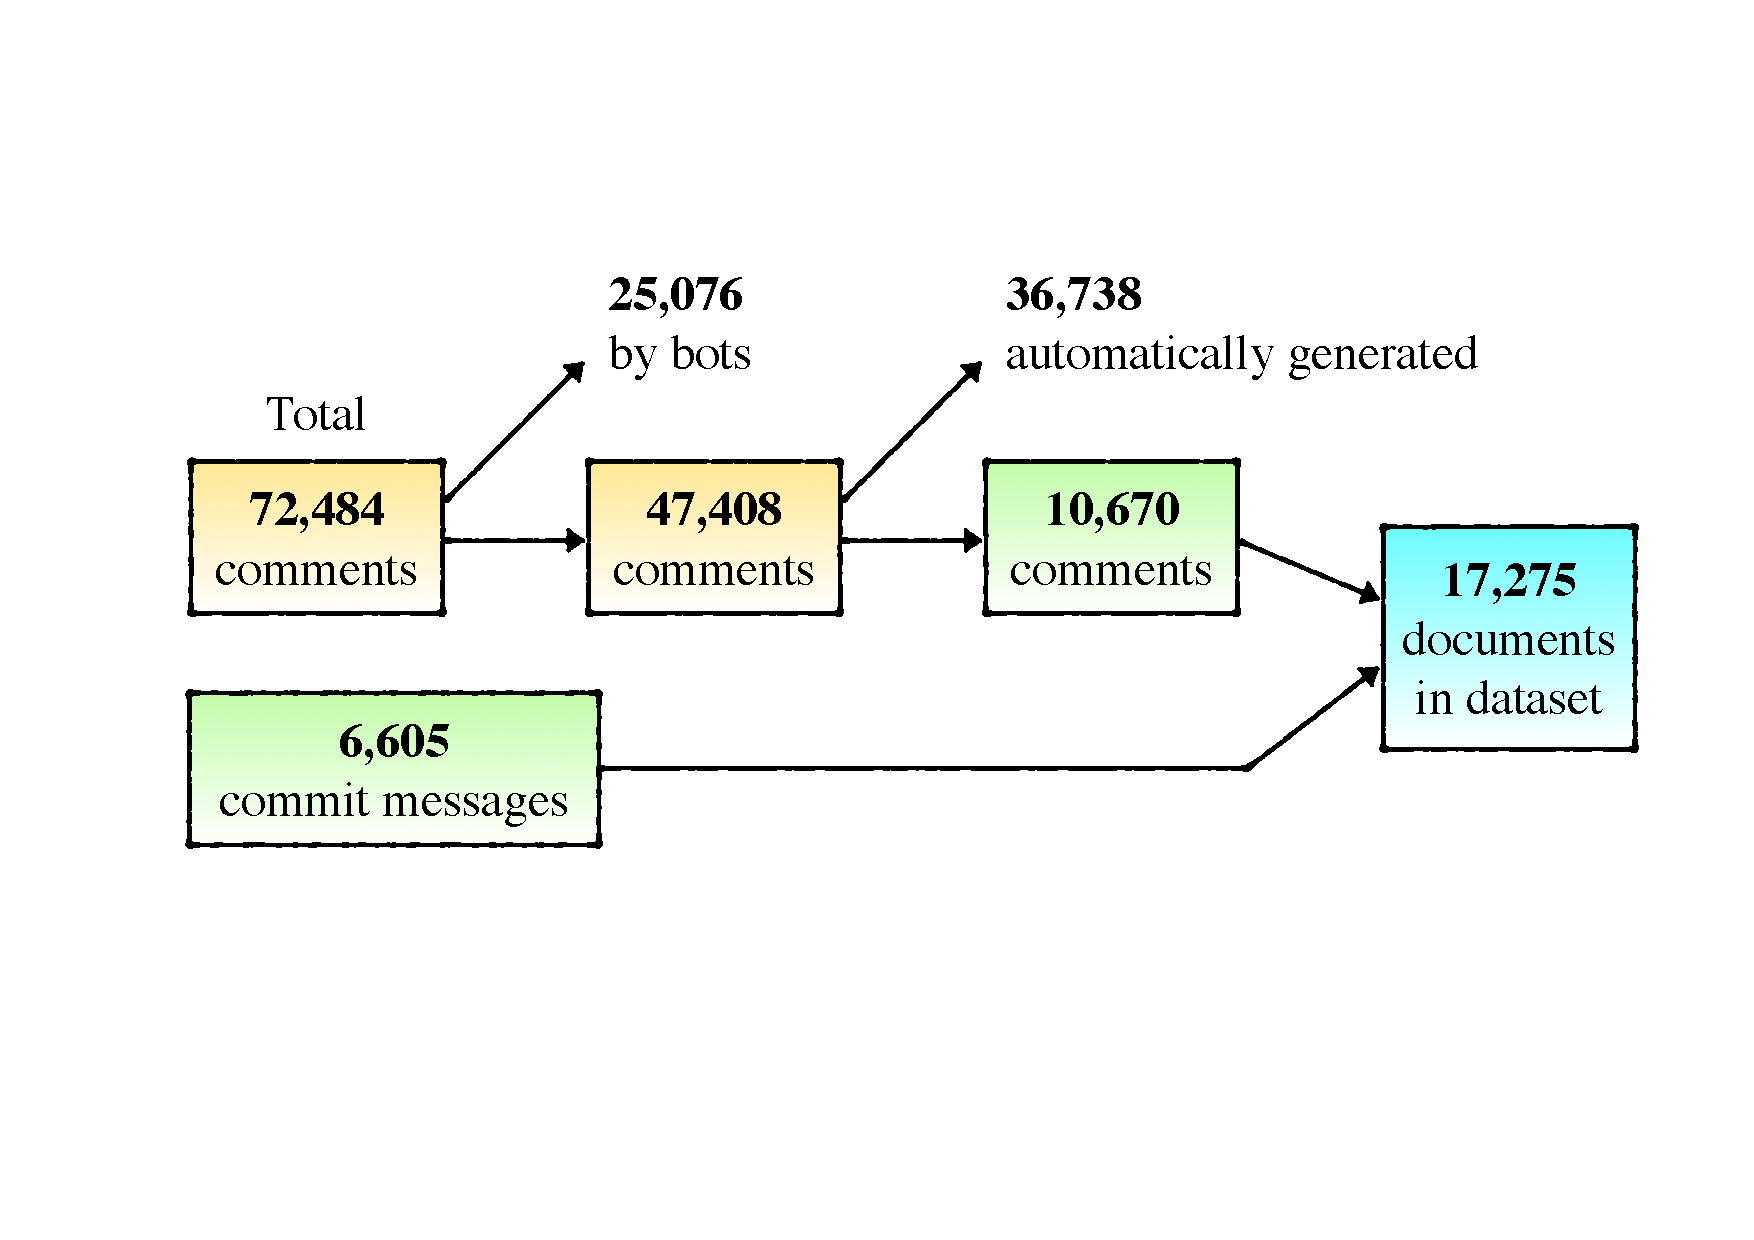
\includegraphics[width=3.2in]{filter}
%\caption{The filtering process.}
%\label{fig:filter}
%\end{figure}
%\subsection{Data Preparation}
%\subsubsection{Data extraction}
%
%6,605 changes and 72,484 comments have been extracted from the raw dataset.
%35\% of the comments are by the system or one of the bots, and are thus discarded.
%
%\subsubsection{Common pattern removal}
%
%By looking for most frequent lines, common patterns were found, such as \emph{`Uploaded patch set 2.'} and \emph{`Change has been successfully cherry-picked to the staging branch as \dots'}.
%
%Removing occurrences of these patterns leaves 77\% of the remaining comments empty.
%This probably means these comments solely contain automatically-generated text, and are thus discarded.
%This leaves us with 10,670 comments and 6,605 commit messages; a total of 17,275 documents.
%
%\subsubsection{Tokenizing}
%
%After the tokenization step, 393,238 tokens are generated in total. They are composed of 20,025 different words.
%This means that each document will be converted into a vector of 20,025 dimensions, each dimension representing a single word.
%

\begin{ResearchQuestions}
\item[RQ1:] Is semantic similarity a good indicator of MCR comment usefulness?
\end{ResearchQuestions}

To answer this question, we randomly sampled 318 comments from our data set and manually identified usefulness as described in previous subsection.
Then, we used these comments for both the training and test data set for our approach to determine its effectiveness.
We also determined the effectiveness of our approach using bootstrapping cross validation:
We randomly selected 90\% of 318 comments for training set and used the remaining 10\% for the validation set.
The performance on the 10\% was measured using precision, recall and F-measure as described in Equation \ref{eq:fmeasure}.
This validation was repeated for 300 times to estimate the mean and variance of the performance.

% \dan{What what the effort in person-hours for this?}
% Thai sez:  Average time per comment is 28 seconds.
%            Since we do a lot of other things while training, it gives us a STDEV of 45 seconds.
%            The median, by the way, is just 10 seconds.

% Since our models do not include unclear type of comments, we defined them as negative condition i.e useless comments in case of useful classification (when using $\Theta(c,S_T,D_T)$ model) and useful comments in case of useless classification (when using $\Omega(c,S'_T,D'_T)$ model).
%\dan{I thought we changed this! It would be bad if we didn't. Let me know what the actual situation is here.}
%
% Thai sez:  We did not. Maybe this is just a matter of wording. I believe what the text says is:
%                - For useful classification, we only look for 3 scored comments.
%                - For useless classification, we only look for 0 scored comments.

From 318 samples, the number of labeled comments were 85, 60, 51, and 122 for 0, 1, 2, and 3 \texttt{YES} votes, respectively.
To estimate similarity and dissimilarity thresholds, we iterated $s_t$, $d_t$, $s'_t$, and $d'_t$ values from every unique similarity and dissimilarity values in our data set.
% \TODO{.......}. 
% \pick{We cannot brute force for every floating number. How did we calculate this?} 
% \dan{I assume Thai used a numerical optimization or root finding routine such as bisection. You iterate until a value is within a given tolerance.}
% Thai sez: answered.
  
Table \ref{tb:thresholds} shows 5 sets of thresholds that best classify useful and useless comments based on F$_1$ score.
% \pick{I used dummy results. Please change it}
\pick{What we got from this table? What information can we interpret? The threshold is slightly different? Is it good or bad? Please describes.} 

\textbf{Model Effectiveness.}
Figure \ref{fig:scatter} shows relationship between comments class and our similarity thresholds.
The green area represents the \emph{useful} classification model $\Theta(c,S_T=0.015529,D_T=2.494944)$, and the red area represents the \emph{useless} model $\Omega(c,S_T=0.087522,D_T=2.265679)$.
This figure also shows an example comment that fall in the different area\pick{Didn't put yet}.

As shown in the figure, most comments falling in green area are useful comments, while very few useless comments fall in this area.
Similarly, most comments in the red area are considered useless.
However, some comments were not determined (in white area).
Some areas of these two models overlap, making results undeterminable.

Table \ref{tb:classify_number} summarizes the number of classification from this results.
Interestingly, 88\% of useless comments classified by our model have \texttt{YES} = 0 and 1 voting scores.
From useful class, a similar proportion is obtained---that most useful comments have \texttt{YES} = 2 and 3 voting scores

\begin{table}[h]
\centering
\small
\caption{Number of comments classified by our approach against ground truth data}
\begin{tabular}{ccccc}
\hline
& \multicolumn{4}{c}{Class from Ground Truth Data} \\ \cline{2-5}
Our&  Useless  & Unclear  & Unclear & Useful \\
Classifications&  (\texttt{YES}=0) & (\texttt{YES}=1) & (\texttt{YES}=2) & (\texttt{YES}=3) \\
\hline \hline
Useless & 69 & 23 & 7 & 6 \\
Useful & 3 & 12 & 24 & 94 \\
Overlap & 1 & 1 & 0 & 1 \\
Undetermined & 12 & 24 & 20 & 21 \\
\hline
\end{tabular}
\label{tb:classify_number}
\end{table}


\begin{table*}[!t]
\caption{An accuracy of similarity and dissimilarity thresholds for useful and useless comment classifications}
\small
\centering
\def\arraystretch{1.2}
\begin{tabular}{ccccccc}
\hline
Prediction Models  & Rank & $s_t$ & $d_t$ & F-measure & Precision & Recall \\ \hline \hline
\multirow{5}{*}{$\Theta(c,S_T=s_t,D_T=d_t)$}
& 1 & 0.015529 & 2.494944 & 0.741 & 0.701 & 0.787 \\ \cline{2-7}
& 2 & 0.015529 & 3.077129 & 0.740 & 0.693 & 0.795 \\ \cline{2-7}
& 3 & 0.016713 & 2.494944 & 0.739 & 0.704 & 0.779 \\ \cline{2-7}
& 4 & 0.015411 & 2.494944 & 0.738 & 0.696 & 0.787 \\ \cline{2-7}
& 5 & 0.015411 & 3.077129 & 0.738 & 0.688 & 0.795
% \\ \cline{2-7}
% & \multicolumn{3}{r}{Average} &  1.00 & 1.00 & 1.00 \\ \cline{2-7}
%& \multicolumn{3}{r}{Min-Max} &   1.00 - 1.00 & 1.00 - 1.00  & 1.00 - 1.00
\\ \hline \hline
\multirow{5}{*}{$\Omega(c,S'_T=s_t,D'_T=d_t)$}
& 1 & 0.087522 & 2.265679 & 0.725 & 0.648 & 0.824 \\ \cline{2-7}
& 2 & 0.087522 & 2.250422 & 0.722 & 0.642 & 0.824 \\ \cline{2-7}
& 3 & 0.087522 & 2.324771 & 0.720 & 0.663 & 0.788 \\ \cline{2-7}
& 4 & 0.052856 & 2.265679 & 0.719 & 0.645 & 0.812 \\ \cline{2-7}
& 5 & 0.087522 & 2.249675 & 0.718 & 0.636 & 0.824
% \\ \cline{2-7}
%& \multicolumn{3}{r}{Average} &  1.00 & 1.00 & 1.00 \\ \cline{2-7}
%& \multicolumn{3}{r}{Min-Max} &   1.00 - 1.00 & 1.00 - 1.00  & 1.00 - 1.00
\\ \hline
\end{tabular}
\label{tb:thresholds}
\end{table*}

\textbf{Model Robustness.} After we performed cross validation, we obtained the following result:
for useful and useless classifications,
we obtained an average F$_1$ score of 0.693 and 0.681,
with standard deviation of 0.090 and 0.118, respectively.
This indicates that we can use our approach to classify with confident of 69.8\%.
\pick{Precision? Recall?} \thai{This is some confidence interval...}

According to the results, we can answer RQ1 that \emph{we can automatically classify usefulness of comments from similarity and dissimilarity using our approach.}

%After we performed cross validation, we obtained the following result:
%for positive and negative classifications,
%we obtained an average F$_1$ score of 0.693 and 0.681,
%with standard deviation of 0.090 and 0.118, respectively.
%This indicates that we can use our approach to classify with confident of 69.8\%.

%After the similarity and distance metrics have been calculated,
%these metrics appear to be able to separate the useful comments from the non-useful ones,
%as can be seen in Fig.\ref{fig:scatter}.
%Note that many comments have a cosine similarity metric of 0.
%This is because the comment text and the corresponding commit message has no word in comment.

\begin{figure}[!t]
\centering
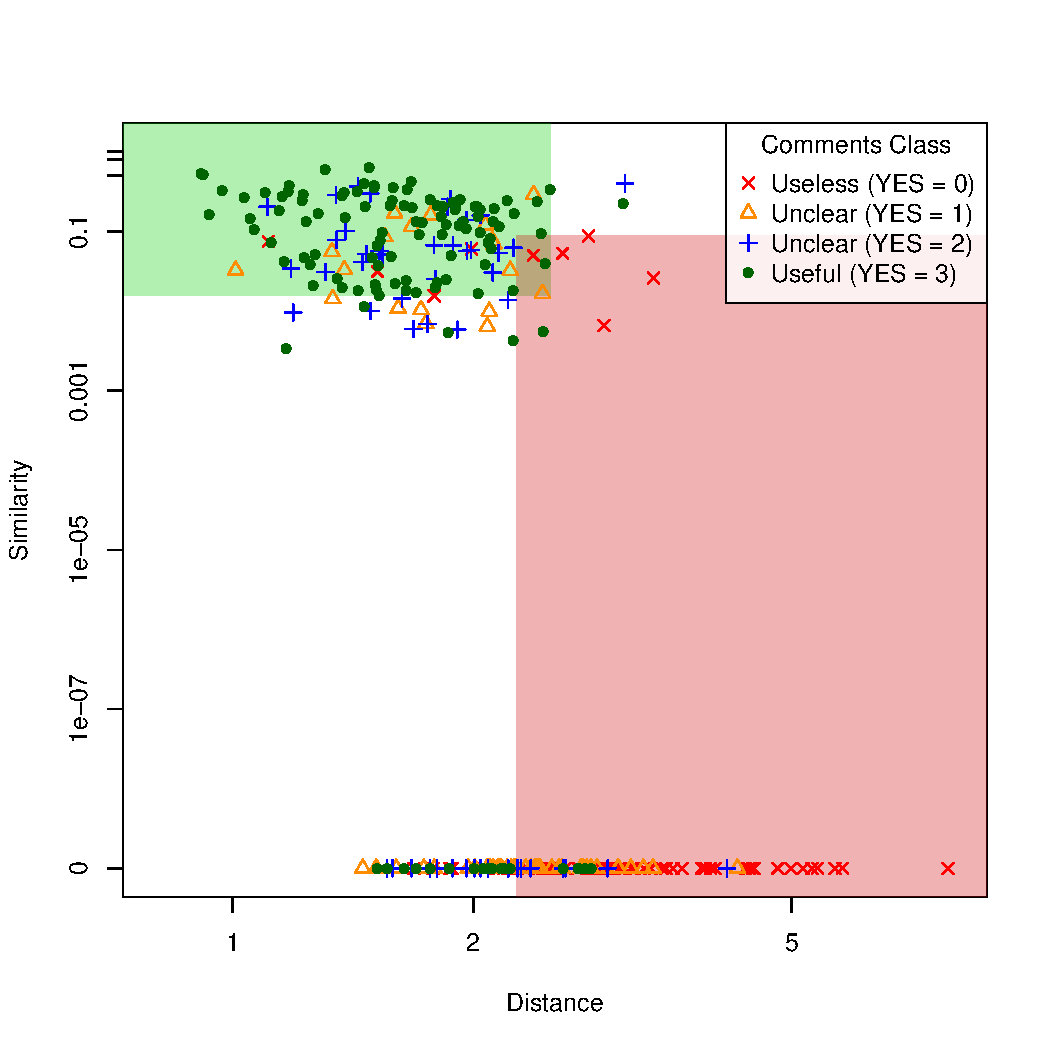
\includegraphics[scale=0.45, trim=0 0 30 50, clip=true]{scatter_log}
\caption{The similarity and distance plot of the training data.
The symbol represents the score, which ranges from 0 to 3.}
\label{fig:scatter}
\end{figure}





\begin{ResearchQuestions}
\item[RQ2:] Is semantic similarity classification cost-efficient, assurable, and scalable?
\end{ResearchQuestions}

To answer this question, timestamps are recorded as three people assess each comment.
Since three people work on their leisure time, there is much variability in the time between each vote.
Therefore, we ignored the time interval between two votes if they are more than 10 minutes apart.

On average, it takes 28 seconds to assess each comment.
However, the median is 10 seconds, suggesting that most comments take only a little amount of time to assess; only few comments take long time.
This also suggests that the time to assess each comment is not normally distributed.
The standard deviation is 45 seconds.

To estimate the total time for us to assess these 318 comments,
we multiplied the average time by the number of comments and the number of people.
This results in 7.42 person hours.

To manually assess all 10,583 comments---even with only one person working at 10 comments per minute---this would take 17.6 person hours.
By running our model through all 10,583 comments, only 2,487 comments receive undetermined result.
That means that about 77\% of the effort is saved.

















